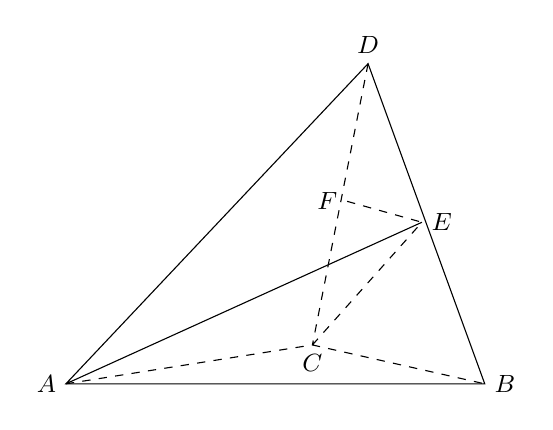
\begin{tikzpicture}[scale=.76, every node/.style={font=\small}]
  \coordinate (A) at (0,0);
  \coordinate (B) at (7,0);
  \coordinate (D) at (5.05,5.35);
  \coordinate (E) at (5.95,2.7);
  \coordinate (C) at (4.12,.65);
  \coordinate (F) at (4.7,3.05);
  \draw (A)--(D)--(B)--cycle (A)--(E);
  \draw[dashed] (D)--(C) (A)--(C)--(B) (C)--(E) (F)--(E);
  \node[left] at (A) {$A$};
  \node[right] at (B) {$B$};
  \node[above] at (D) {$D$};
  \node[right] at (E) {$E$};
  \node[below] at (C) {$C$};
  \node[left] at (F) {$F$};
\end{tikzpicture}
